\documentclass[a4paper,11pt]{article}
\usepackage{graphicx,fancyhdr,clrscode,wrapfig,tabularx,amsmath,amssymb,enumerate,amsthm}
\usepackage[usenames, dvipsnames]{color}
\usepackage[pdftex,colorlinks,linkcolor=Black]{hyperref}
\usepackage[left=2cm,top=2cm,right=2cm,bottom=2cm,nohead]{geometry}

\theoremstyle{definition} \newtheorem{definition}{Definition}

\raggedbottom
\begin{document}

    \begin{center}
    {\Large OGO 2.1 fall 2009}\\[0.25cm]
    {\bf \Huge Curve Reconstruction}\\[0.75cm]
    \begin{tabular}{p{3cm}p{3cm}p{3cm}p{3cm}p{3cm}}
    E.I.R. van Delden & T. Hermans & T. van der Hoek & J. Sijen & R. Wolffensperger\\
    (0618959) & (0664881) & (0655570) & (0652478) & (0612853)
  \end{tabular}
    \end{center}

    \begin{abstract}
      This report is about reconstructing a curve from of a set of given points. We have created three different algorithms to solve the four given problems. \emph{ImprovedNearestNeigbor} is used to solve open and closed curves, \emph{DirectedNearestNeighbor} is used to solve all intersecting curves and \emph{UpToFiveSort} solves curves that consists of two to five, non-intersecting, curves. These algorithms run, respectively, in $O(n^{2}), O(n^{2})$ time, both theoretically and in practice. \emph{UpToFiveSort} theoretically runs in $O(n^{3})$, but in practice in $O(n)$. We have also tested and evaluated each of our algorithms, in which we concluded that we can solve most, but not all, test cases within the given time of 5 minutes.
    \end{abstract}

\section{Introduction}
\label{sec:Introduction}
In today's world 3D Scanners are being used for a wide variety of applications, most commonly for making 3D models for archiving purposes, or to use in the production of video games or movies.
To make such a 3D model these scanners measure a great number of points on the surface of an object, these points together are called point clouds. On such a point cloud an algorithm is applied to reconstruct the object to make the actual 3D model.
2D reconstruction does the same but only in a two dimensional form. So the points only consist of $x$ and $y$ coordinates.
\\
In this paper we are going to look at the problem of reconstructing 2D curves from a given set of points. This is an important subject in today's world; 2D scanners are being used for a wide variety of applications, most commonly for making 2D models for archiving purposes. To make such a 2D model these scanners measure a great number of points on the surface of an object, these points together are called point clouds. On such a point cloud an algorithm is applied to reconstruct the object to make the actual 2D model.\\ \\
We have designed, implemented and tested an algorithm to solve the different curves of the given problems. We have repeated this process after each batch of experiments, using the results of those experiments to improve our algorithm. Testing the algorithms was done on a number of testcases, using a visualizer to check the resulting curve, and keeping track of the running time of the algorithm.\\ \\ \\
The results of our development are the algorithms \textit{NearestNeighbor}, the improved versions \textit{DirectedNearestNeigbor} and \textit{ImprovedNearestNeighbor} and \emph{UpToFiveSort}. \\
\textit{NearestNeighbor} searches for the nearest neighbor of the input points and connects them to reconstruct the curve. It does so in $O(n^{2})$, both theoretically and in practice. \\
\textit{DirectedNearestNeighbor} searches for the point within a certain range which differs the least in direction of the currently constructed curve. \emph{DirectedNearestNeigbor} run in $O(n^{2})$ For the self-intersecting curves this is a good solution, but for the other cases \textit{ImprovedNearestNeighbor} and \textit{UpToFiveSort} proved to be better. \\
\textit{ImprovedNearestNeighbor} searches for the nearest neighbor of the input points until it's back at the starting point and then inserts all the points it skipped in an already existing curve. \emph{ImprovedNearestNeighbor} also runs in $O(n^{2})$. \\
 \textit{UpToFiveSort} uses \textit{ImprovedNearestNeighbor} to make multiple curves. When the curve is back at its starting point, the next curve is constructed with (some of) the remaining points, and continues on until there are no points left. When there are more than five curves constructed, the smallest curves are inserted into the nearest curve. The running time of \emph{UpToFiveSort} is the most curious, it's theoretical runnning time is $O(n^{3})$, but during our tests it ran in $O(n)$. \\
In our conclusion we revisit the results of our experiments and determine what algorithms are needed to solve any of the curve reconstruction problems.

\subsection{Overview of this document}
\label{sec:overview_of_this_document}
This report has three parts; our algorithms, our experiments with both discussions about our visualizer and the algorithms and our concluding remarks on the process of implementing a 2D-reconstruction algorithm.\\
The outline of each algorithm is as follows:
\begin{itemize}
    \item Additionally used functions
    \item Needed definitions
    \item Proof of Correction
    \item Running time analysis
\end{itemize} 
\section{Description of the algorithms}
\label{sec:Description}

\subsection{Nearest Neighbor}
\label{sub:nearest_neighbor}

Our initial approach was to solve the reconstruction of the curve using only  the nearest neighbor property.\\
We begin with discussing some functions on which our algorithm relies, then we give a description, analysis and test results of the algorithm itself.\\

  \noindent\large\textbf{Lexicographic Smallest}\\
    We introduce \textit{LexicographicSmallest} to find the lexicographic smallest point in a set of points. This will be the point from which the curve reconstruction starts. Finding this point is needed for all types of curve problems.
    To find the lexicographic smallest point in a set we go through the array keeping track of the lexicographic smallest point found so far. Because all points are unique, there exists exactly one lexicographic smallest point in the array.\\
    The running time of this function is $O(n)$, because after each of $n$ points in the array is checked, the lexicographic smallest point is found.\\

  \noindent\large\textbf{Nearest Neighbor}\\
    Our algorithm assumes the following definition:
        \begin{definition} \label{def:nn}
          Given a set $S$ of $n$ input points, the nearest neighbor of a point $p$ is the point $q$ with the smallest distance to $p$ from all points in $S$.
        \end{definition}
    \noindent \emph{NearestNeighbor} is initially called with an array $S$ of $n$ points and one empty array $B$ which has the same length.\\
      From $S$ the lexicographic smallest point is chosen, say $p$. This point $p$ is removed from $A$ and placed into $B$. $p$ is the point from which we start looking for the nearest neighbor. All the lengths between this point and all the remaining points in $A$ are measured and the point with the smallest distance to this point is chosen as to be the nearest neighbor, say $q$.\\
      Now that the nearest neighbor of $p$ is found, $q$ is moved from $A$ to $B$. Then the nearest neighbor for $q$ is found. This process continues until all points except for the last one in $A$ are processed. This point has no nearest neighbor anymore, so is directly moved from $A$ to $B$. When $A$ is empty and $B$ full, $B$ is returned.

      \begin{center}
        \begin{tabular}{l l }
                  & \textbf{NearestNeighbor}$(P)$                                                \\
              01  & $ls \gets$ \textbf{LexicographicSmallest}$(P)$                               \\
              02  & $p \gets P[ls]$                                                              \\
              03  & \textbf{for} $i \gets 0$ \textbf{to} $|P| - 2$ \textbf{do}                   \\
              04  & \qquad $P \gets P \backslash \{ p \}$                                        \\
              05  & \qquad $d \gets \infty$                                                      \\
              06  & \qquad $q \gets p $                                                          \\
              07  & \qquad \textbf{for} $j \gets 0$ \textbf{to} $|P| - 1$ \textbf{do}            \\
              08  & \qquad \qquad \textbf{if} \textbf{distance}$(p, P[j]) < d$ \textbf{then}     \\
              09  & \qquad \qquad ~~ $d \gets$ \textbf{distance}$(p, P[j])$                      \\
              10  &  \qquad \qquad ~~ $q \gets P[j]$                                             \\
              11  &  $S \gets S \cup \{ p \}$                                                    \\
              12  &  $p \gets q$                                                                 \\ \hline
          & \qquad \qquad \qquad \qquad\textbf{Total } \qquad\qquad $O(n^{2})$
         \end{tabular}
         \label{fig:nn_pseudo_code}\\
         Figure 2.1: Pseudo code for \textit{NearestNeighbor}
      \end{center}

    \noindent\textbf{Proof of Correctness}\\
        \textit{To prove:} \textit{NearestNeighbor} finds for each point in the set $S$ its nearest neighbor.\\
        \textit{NearestNeighbor} begins with removing $p$ from $S$ and calculates the distances between this point $p$ and the other points in $S$ and keeps track of the smallest point processed so far.\\
        So when all points are processed \textit{NearestNeighbor} has found the nearest of point $p$, say $q$.Then the algorithm computes the nearest neighbor of $q$, say $r$, in the same way as for $p$ and removes $q$ from $S$.\\ Every time the nearest neighbor of a point is found, the found point is removed from $S$.
        This goes on until the $n-1^{th}$ point is processed; the nearest neighbor of this point is the only point left in set $S$ point $n$. Point $n$ only has a next nearest neighbor in a closed curve problem, namely the starting point. In an open curve problem, it has no new nearest neighbor. \\

    \noindent\textbf{Running Time Analysis}\\
        Proving the running time for \textit{NearestNeighbor} is straight forward. There are only three lines that are not constant time; lines 1, 3 and 7 in Figure 2.1.\\
        Line 1 uses a function that searches for the lexicographic smallest for its given input set. This takes $O(n)$ time.\\
        Line 7 starts a for loop that looks through all remaining elements in the set $P$ looking for the smallest distance between point $j$ and given point $p$. This comparison is done in constant time and does not affect the running time of the for loop. In the first run, this for loop needs to go through the most number of elements, namely $n-1$ elements. The running time of this loop is $O(n)$. \\
        Line 3 starts the for loop that runs through all elements in the set, minus the last element. Thus, this takes $O(n-1)$. We need to take into account the nested for loop and finding the lexicographic smallest point, this makes the total running time: \\
        $O(n-1) * O(n) + O(n) =  O(n^{2} - n ) + O(n) = O(n^{2})$ \\
        Thus \textit{NearestNeighbor} runs in $O(n^{2})$. 
\subsection{Directed Nearest Neighbor}
\label{sub:directed_nearest_neighbor}
To improve the nearest neighbor algorithm we will not only search for the nearest neighbor but also look at the direction we are going while constructing the curve, and look for more points in the vicinity. Now it is not always the case that the nearest neighbor of a certain point is chosen, but the point which differs the least in direction from the previous edge from all other points within a certain range.
Again we begin with giving some functions on which our algorithm relies, such as searching for points and determining the direction, then we give a description of the algorithm itself.\\

 \noindent\textbf{Lexicographic Smallest}\\
    We again need to look for the lexicographic smallest point in the point cloud and thus reuse.\\

  \noindent\textbf{Find Points In Range}\\
    \textit{FindPointsInRange} is introduced to find points within a certain range (using the distance of the previous edge and a constant multiplier) from a specific point. The result of this function is used in the function \textit{GiveBestPoint}.
    \noindent\emph{FindPointsInRange} finds all points which lie in a certain range $\alpha$ and is called with three parameters: one for the range, one for a point, $p$, and one for the array $S$ with all the points that need to be checked. In the function a new array $R$ is defined which is used to store all points in the range. Now, for all points in $S$, the distance between $p$ and a point in $S$, say $x$, is compared to the range. If the distance is smaller than the range, point $x$ is added to $R$. When all points in $S$ are processed, $R$ is returned.\\
    From this description we can conclude the following definition:\\
      \begin{definition} \label{def:fpir}
          Given the range $\alpha$, the point from which to look, say $p$, and the set of points which still need to be processed, say $S$, then for all points in $S$ holds that a point $q$ is returned if and only if $q$ lies within range $\alpha$ from $p$.
      \end{definition}
    \noindent\emph{FindPointsInRange} consists of a single for loop that goes through all of its inputs elements. In the for loop is a single if statement, that checks the distance between the given point and the current point. If the current point is within the given range, it is added to the solution.
    This takes $O(n)$ time.\\

  \noindent\textbf{Give Best Point}\\
     This function returns the point which, when connected to the current curve, differs the least in direction of the current curve's direction. It is called on a array $S$ of $n$ points, where the first point is called $p$, the second $q$ and the rest $[1,2,3 \ldots Count-2]$. First the angle of the edge between $p$ and $q$, say $\alpha$, is computed, then the angle between $q$ and $1$. This angle, $\beta$, is compared to $\alpha$ and the point $1$ is stored as the best point so far. Now the rest of the points are processed comparing each angle to the one of the best point so far. When all points in $S$ have been checked the best point is returned.\\
     Our definition of the best point is given below.\\
      \begin{definition} \label{def:gbp}
          Given the edge $(p,q)$ and the set $S$, with $S$ being the $n$ points within range $\alpha$ from $q$, point $r$ in $S$ is returned if and only if the angle of the edge $(q,r)$ differs the least from the angle of the preceding edge $(p,q)$. This returned point is called the ``best point''. (All angles are with respect to the x-axis).
      \end{definition}
      \noindent \emph{GiveBestPoint} consists of a single loop that goes through all of its inputs elements, and several if statements. \textit{GiveBestPoint} first calculates the angle of it's first line segment than goes into the for loop. The for loop goes through all other points, makes the line segment, calculates the angle and compares it with the current best (and replaces if so). After the for loop it returns the solution.\\
      Because only the for loop takes longer than constant time, the running time of \textit{GiveBestPoint} is $O(n)$\\

    \noindent\textbf{Insert Lost Points}\\
        \noindent\emph{InsertLostPoints} inserts all lost points on the best spot in the solution array $S$, which contains the currently connected points in order, and is initially called with an array of lost points, say $B$. For every point in $B$ its nearest neighbor is searched for in array $S$. The index $i$ of each nearest neighbor is stored, the distance between $p$ and $S[i-1]$ is stored in $v$ and the distance between $p$ and $S[i+1]$ in $w$. Next $v$ is compared to $w$, if $v$ is smaller or equal to $w$, $x$ is inserted at $S[i]$ in $S$, else $x$ is inserted on $S[i+1]$ in $S$. After all points are inserted ($B$ is empty) $S$ is returned.\\
        Our definition of a lost point point is as follows:\\
        \begin{definition} \label{def:ilp}
          A lost point is a point that is not in the curve, after using the Nearest Neighbor algorithm.
        \end{definition}
        \textit{InsertLostPoints} is given two sets; the solution set, say $SOL$, so far and a set containing the points that have been skipped, say $LPS$. Now for each point in $LPS$, say the point $p$, the distance is calculated between $p$ and each point in $LPS$. The smallest distance is saved, a decision is made where our point $p$ needs to be inserted and is then inserted.\\
        The running time of \textit{InsertLostPoint} is determined by the amount of points in $LPS$, say $n$ points, the number of points in $SOL$, say $k$ points and inserting a point into an array. Determining the closest point takes $O(k)$ time, inserting takes $O(k)$ time. These two operations are run in a for loop that takes $O(n)$ time, so the running time of \textit{InsertLostPoint} takes $O(n*(2k)) = O(n*k)$ time.\\
        \emph{Note: Because of the nature of this function, the solution set will probably be bigger than the set of points that still need to be inserted. This makes this function mostly dependent on the number of points already inserted. The worst case scenario would have both sets of equal size, taking $O(n^{2})$ time.}\\

  \noindent\large\textbf{Directed Nearest Neighbor}\\
        \textit{NearestNeighbor} had a lot of zigzagging in its resulting curve, by adding direction to this algorithm we tried to solve this problem. \textit{DirectedNearestNeighbor} constructs a curve with as least changes of direction as possible, so there's no zigzagging anymore, but a straight line.\\
        To accomplish this we look in a certain range from a specific points for points and choose the point in that range which differs the least in direction from the current curve.\\
        In comparison to \textit{NearestNeighbor} (\ref{sub:nearest_neighbor}) one more array $C$, which is initially empty, is used. Finding the first and second point of the solution stays the same and both points are moved from $A$ to $B$. From those two points we calculate the range, which is the distance between them multiplied by a constant $c$. Now the function \textit{FindPointsInRange} is called with three parameters: the range, $\alpha$, the last point in our solution, $p$, and the array $A$. According to Definition~\ref{def:fpir} all points in $A$ which lie within range $\alpha$ from the $p$ are returned. Those points are stored in $C$. If there are less than two points in $C$ the \textit{NearestNeighbor} is called. When there two points or more the two points stored in $B$ are moved to $C$, making sure those points are the first two points in $C$, then \textit{GiveBestPoint} is called with parameter $C$. From Definition~\ref{def:gbp} this function returns the point that, when connected to the current curve, differs the least from the direction of the preceding edge. This point is added to $B$ and deleted from $A$. These steps will be repeated until the point we started from is connected to the curve. Then \textit{InsertLostPoints} is called to insert the skipped/lost points in the curve. When this is done the curve is constructed.

        \begin{center}
        \begin{tabular}{ll}
       & \textbf{DirectedNearestNeighbor}$(P)$\\
        01     & $ls,p,beginpunt \gets $\\
               & ~~\textbf{LexicograhicSmallest}$(P),P[ls],P[ls]$\\
        02     & \textbf \textbf{repeat}\\
        03     & \qquad $P,skip \gets P \backslash \{ p\},false$\\
        04     & \qquad \textbf{if} $|A| \geq 2$ \textbf{then}\\
        05     & \qquad \qquad $skip \gets true$\\
        06     & \qquad \qquad $r \gets \alpha * d(A[|A|-1],A.last)$\\
        07     & \qquad \qquad $B \gets$\\
               & \qquad \qquad ~~\textbf{FindPointsInRange}$(P,p,r)$\\
        08     & \qquad \qquad \textbf{if} $|B| = 0$ \textbf{then}\\
        09     & \qquad \qquad \qquad $skip \gets false$\\
        10     & \qquad \qquad \textbf{elseif} $|B| = 1$ \textbf{then}\\
        11     & \qquad \qquad \qquad $q \gets B[0]$\\
        12     & \qquad \qquad \textbf{else}\\
        13     & \qquad \qquad \qquad $B \gets \{A.last\} \cap$\\
               & \qquad \qquad \qquad ~~$\{A[|A|-1]\} \cup B$\\
        14     & \qquad \qquad \qquad $q \gets$ \textbf{GiveBestPoint}$(P)$\\
        15     & \qquad \textbf{if} \textbf{not} $skip$ \textbf{then}\\
        16     & \qquad \qquad $r,q \gets \infty,p$\\
        17     & \qquad \qquad \textbf{for} $j \gets 0$ \textbf{to} $|P| - 1$ \textbf{do}\\
        18     & \qquad \qquad \qquad $c \gets d(p,P[J])$\\
        19     & \qquad \qquad \qquad \textbf{if} $c < r$ \textbf{then}\\
        20     & \qquad \qquad \qquad \qquad  $r,q \gets c, P[j]$\\
        21     & \qquad $A,p \gets A \cup {q},q$\\
        22     &\textbf{until} $p = beginpunt$\\
        23     &  \textbf{if} $|P| > 0$ \textbf{then}\\\
        24     &  \qquad \emph{InsertLostPoints(P,A)}\\ \hline
       &  \qquad \qquad \qquad \qquad \textbf{Total } \qquad\qquad$O(n^{2})$
        \end{tabular}
        \label{fig:dnn_code}\\
        Figure 2.2: Pseudocode for \textit{DirectedNearestNeighbor}
      \end{center}

     \noindent\textbf{Proof of Correctness}\\
     \textit{To prove:} \textit{DirectedNearestNeighbor} makes a curve with as least changes of direction as possible.
      For a point in $S$ \textit{DirectedNearestNeighbor} chooses the next point such that it lies with the least change of direction from the edge you came from (see Definition~\ref{def:gbp}). \textit{DirectedNearestNeighbor} does this for all points in $S$, except for the first two points; the first point is found with \textit{LexicographicSmallest} and connected to the second by using \textit{NearestNeighbor}. Because from here on all points are chosen with the least change of direction to its preceding edge, the resulting curve will contain as least changes of direction as possible on the points processed so far. At the last step lost points are inserted at the right spot in the set by the function \textit{InsertLostPoints}. Because they are inserted in between their nearest neighbor and their second nearest neighbor the curve will still contain as least changes of direction as possible when all points are part of the curve.\\

    \noindent\textbf{Running Time}\\
       The overall running time of \textit{DirectedNearestNeighbor} is determined by three function calls and two loops. We will first explain the factors of consequence, then what situations there are that define the running time.
       \textit{DirectedNearestNeighbor} uses two loops, the first is a for loop on line 2 and goes through $n-1$ input elements. The second is a repeat loop on line 19 and takes $O(n-1)$ time, but is not run for each iteration, only for the first and last element. \\
        There are three sub functions that have each have a running time of $O(n)$, \textit{LexicographicSmallest}  \textit{FindPointsInRange} and \textit{GiveBestPoints}. Only \textit{FindPointsInRange} and \textit{GiveBestPoints} are nested in the main for loop and are thus of consequence.\\
        There are two main scenario's when running \textit{DirectedNearestNeighbor}:\\
        \begin{itemize}
          \item We are either looking at the first or the last input element.
          \item We are processing any other input element.
        \end{itemize}
         The first situation is the same as running our first \textit{NearestNeighbor} and is done in $O(n^{2})$, it's the second case that has been changed.\\
         \textit{FindPointsInRange} is always run in this situation, taking $O(n)$ time. It is followed by an if statement, that calls the function \textit{GiveBestPoint} that also runs in $O(n)$. Finally the function \textit{InsertLostPoints} is called which has a running time of $O(n^{2})$, so the total running time is: \\
             $O(n) + (O(n-1)*(3O(n))) + O(n^{2}) = O(n) + (O(n^{2} - 3n)) + O(n^{2}) = O(n^{2} - n) + O(n^{2}) = O(n^{2})$ \\ \\
          Thus, the running time is still $O(n^{2})$. Though, in practice, it will be slightly slower than our first algorithm, because there are three additional function calls of $O(n)$ time, instead of one. 
\subsection{Improved Nearest Neighbor}
\label{sub:improved_nearest_neighbor}
Although the \textit{DirectedNearestNeighbor} gave better results in some test-cases (especially self-intersecting curves) than \textit{NearestNeighbor}, there were a lot of test-cases in which the resulting figure was far worse than the one \textit{NearestNeighbor} constructed. Therefore we continued to improve \textit{NearestNeighbor} and we use \textit{DirectedNearestNeighbor} only for the self-intersecting curve reconstruction.\\
\textit{ImprovedNearestNeighbor} relies on two new functions: the first one adds the functionality of inserting points at the end, this way there are no connections between a point on one side of the canvas and one on the other side, the second is used for making open curves. This deletes the longest edge in a closed curve and reorders the set of points accordingly.\\
A more detailed description of these two functions is given below, followed by a description of \textit{ImprovedNearestNeighbor}\\

 \noindent\textbf{Lexicographic Smallest}\\
    We again need to look for the lexicographic smallest point in the point cloud and thus reuse.\\

  \noindent\textbf{Insert Lost Points}\\
    For \textit{ImprovedNearestNeighbor} we also need to insert lost points.\\

  \noindent\textbf{Make Open Curve}\\
    For creating an open curve we use the following definition:\\
    \begin{definition} \label{def:moc}
        To create an open curve the edge between two points that is the longest of all edges in a closed curve has to be removed.
    \end{definition}
    \textit{MakeOpenCurve} is used to find and create the opening in a closed curve. The array $Points$ that has already been ordered by \textit{ImprovedNearestNeighbor}, and thus is a closed curve, is given to \textit{MakeOpenCurve}. For each point in the array $Points$ the distance between two consecutive points is determined and compared to the last distance. The index of the starting point of the longest edge is saved, say the point $lp$. \\
    If $lp$ is the last point in the array $Points$, we have the correct open curve. If it is not the last point the array must be reordered. The lexicographic smallest of the two endpoints is determined. \\
    If this not the last point in the array, but the lexicographic smallest endpoint is the first point in the array $Points$, then the lexicographic smallest is put into the array $results$ followed by the second end point. Then all other points are added in reverse order.\\
    If $lp$ is not the last point, and the lexicographic smallest endpoint is not the first point, all points from and including the endpoints are added to the front of the $results$ array. Then the points from start to the opening are added to the $results$ array, which is then returned.\\
    This function is only called when the input curve-type is an open curve.\\
    To show \textit{MakeOpenCurve} actually makes an open curve the following proof is given:\\
    \textit{ImprovedNearestNeighbor} first makes a closed curve of the input points, then \textit{MakeOpenCurve} measures the length of all edges and the longest one is removed. There always exists a longest edged, so after \textit{MakeOpenCurve} has removed this edge, an open curve is created.\\

    \noindent\textbf{Improved Nearest Neighbor}\\
        This function is an improvement on the original Nearest Neighbor and is used for closed curves.\\
        The function first determines the \textit{LexicographicSmallest} point $p$. Then this \emph{ImprovedNearestNeighbor} starts to search for the point $q$ with the smallest distance, to $p$ the starting point. If $q$ is not the starting point it adds it to list of points $Result$. $p$ becomes $q$ and from point $q$ with the smallest distance to $p$ is determined and added into the $Result$ list if $q$ is not the starting point. This is repeated until the starting point is seen again. Lastly there is a check to see if there are any loose points left. If this is the case, the function \textit{InsertLostPoints} is called with the parameters $P$ and the $Result$ list to insert the lost point. \\

        \begin{center}
        \begin{tabular}{l l l}
           & \textbf{ImprovedNearestNeighbor}$(P)$                           & \\
         01 & $ls,p \gets $ \textbf{Lexicographic-}                          &\\
            & ~~\textbf{Smallest}$(P),P[ls]$                                & $O(n)$ \\
         02 & $start, loopcount \gets p,0$                                   &  \\
         03 & \textbf{repeat}                                                & $O(n^{2})$ \\
         04 & \qquad $loopcount \gets$                                        & \\
            & \qquad ~~$loopcount +1$                                            & \\
         05 & \qquad $P \gets P \backslash \{ p\}$                            & \\
         06 & \qquad \textbf{If} $loopcount = 5$ \textbf{then}               & \\
         07 & \qquad \qquad $P \gets P \cup \{ start\}$                          &  \\
         08 & \qquad $q,d \gets p, \infty$                                   &\\
         09 & \qquad \textbf{for} $j \gets 0$ \textbf{to} $|P| - 1$          & $O(n)$\\
         10 & \qquad \qquad $c \gets d(p,j)$                                 & \\
         11 & \qquad \qquad \textbf{if} $c < d$ \textbf{then}                & \\
         12 & \qquad \qquad \qquad $d,q \gets c,P[j]$                        & \\
         13 & \qquad \textbf{if} $q \neq start$ \textbf{then}                & \\
         14 & \qquad \qquad $Result \gets$                                   &\\
            & \qquad \qquad ~~$Result \cup \{q\}$                 & \\
         15 & \qquad $p \gets q$                                             & \\
         16 & \textbf{until} $p = start$                                     & \\
         17 & \textbf{if} $|P| > 0$ \textbf{then}                            & \\
         18 & \qquad \textbf{Insert-}                                       & \\
            & \qquad ~~\textbf{LostPoints}$(P, Result)$                  & $O(n^{2})$\\
         \hline
         & \qquad\qquad\qquad\qquad\textbf{Total:} & $O(n^{2})$
         \end{tabular} \\
         Figure 2.3: Pseudo code for \textit{ImprovedNearestNeighbor}
         \end{center}
    \noindent\textbf{Proof of Correctness}\\
        \textit{To prove:} \textit{ImprovedNearestNeighbor} makes a closed curve.\\
        \textit{ImprovedNearestNeighbor} uses the function \textit{LexicographicSmallest} to determine the starting point, then when the input curve-type is closed, it makes a curve by using \textit{NearestNeighbor}. After the curve is created, it calls \textit{InsertLostPoints} to insert points that are skipped by \textit{NearestNeighbor}. From Definition~\ref{def:ilp} we know that after \textit{InsertLostPoints} is finished no lost points are left and inserted on the correct place in the solution.
        So \textit{ImprovedNearestNeighbor} makes one closed curve of all input points.\\

    \noindent\textbf{Running Time Analysis}\\
    	The analysis of \textit{ImprovedNearestNeighbor} bears much resemblance to that of \textit{NearestNeighbor}. Line 1 finds the lexicographic smallest point, taking $O(n)$ time. Line 7 has a for loop, going through the remainder of points. The contents of the loop all take constant time, so the loop itself takes $O(n)$. The for loop is included in the repeat until loop on line 3, which, in the worst case, loops through all points. Since the running time of the body of this repeat until loop is $O(n)$, and it loops at most $n$ times, the total running time of this loop is $O(n^2)$. Now, the only real difference with \textit{NearestNeighbor} is the addition of the \textit{InsertLostPoints} function, which has a running time of $O(n^2)$. (Note that we proved this before.) The total running time is therefore:
		$O(n) + O(n^{2}) + O(n^{2}) = O(n^{2})$ \\

\chapter{Up To Five Sort}
\label{cha:up to five sort}


  \section{Lexicographic Smallest}
  \label{sec:utfs_lexicographic_smallest}
    LexicographicSmallest was not changed for ImprovedNearestNeigbor, for analysis of this function see \ref{sec:nn_lexicographic_smallest}.

  \section{Insert Lost Points}
  \label{sec:utfs_insert_lost_points}

    \subsection{Definitions}
    \label{sub:ilp_definitions}
        \begin{definition} \label{def:ilp}

        \end{definition}

    \subsection{Functional Description}


    \subsubsection{Proof of Correctness}
    \label{ssub:ilp_proof}

    \subsection{Running Time Analysis}
    \label{sub:ilp_running_time_analysis}

  \section{Up To Five Sort}
  \label{sec:up to five sort}

    \subsection{Definitions}
    \label{sub:utfs_definitions}
      \begin{definition} \label{def:inn}

      \end{definition}

    \subsection{Functional Description}
    \label{sub:utfs_functional_description}


    \subsubsection{Proof of Correctness}
    \label{ssub:utfs_proof}

    \subsection{Running Time Analysis}
    \label{sub:utfs_running_time_analysis}


  \section{Test Results}
  \label{sec:utfs_test_results}
    \subsection{Running time}


        \begin{table}[!h!b!p]
        \begin{center}
          \begin{tabular}{|p{2.5cm}|p{2.5cm}|}
              \hline
              Points & Seconds\\
              \hline
              \hline
              500 & 0.015\\
              \hline
              1000 & 0.031\\
              \hline
              1500 & 0.041\\
              \hline
              2000 & 0.078\\
              \hline
              5000 & 0.390\\
              \hline
              10000 & 1.747\\
              \hline
              15000 & 5.008\\
              \hline
              20000 & 8.783\\
              \hline
              30000 & 20.951\\
              \hline
              40000 & 25.053\\
              \hline
              50000 & 53.991\\
              \hline
              60000 & 71.230\\
              \hline
              80000 & 139.543\\
              \hline
          \end{tabular}
          \label{tab:utfs_runningtime}
          \caption{Results of testing ImprovedNearestNeighbor}
        \end{center}
      \end{table}


        \begin{figure}
          \begin{center}
            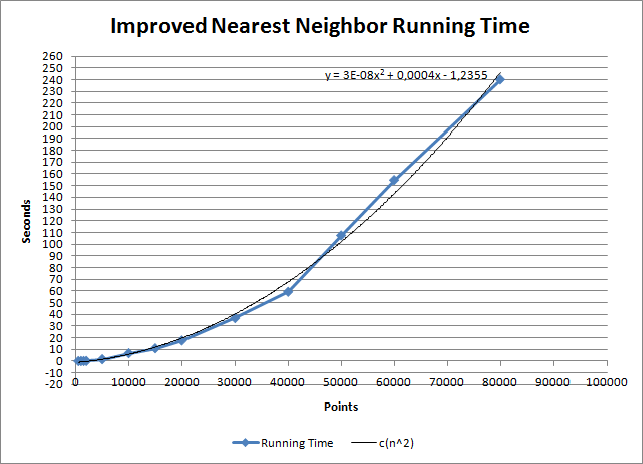
\includegraphics[scale = 0.7]{3ImprovedNearestNeighbor/innRuntimeGraph.png}\\
            \caption{Graph of Improved Nearest Neighbor Running Time}
            \label{fig:inn_runnningtime}
          \end{center}
        \end{figure}

      \noindent The results of the running

    \subsection{Correct output}


   \subsection{Conclusion from tests} 

\section{Experimental Evaluation}
\label{par:Discussion}

\subsection{Visualizer}
\label{sec:Vizualizer}
In order to make the debugging more easier we developed a visualization program, ``CurveReconDriver''. CurveReconDriver is a multi-platform program that runs on Windows, Linux and Mac OS X. With this program we can draw points or let the program generate a given number of random points. The feature set of CurveReconDrive also includes the importing and exporting of test cases, from which to generate curves. This program is very useful to detect errors in our different implementations, because it helps to visually see the wrong decisions our algorithms made.\\
We ran a number of test-cases to test our algorithms. The test-cases were generated using our visualization program, which has the ability to draw points. This enabled us to easily generate test-cases and test them using the same program. Since the visualization program automatically draws the algorithm's output, errors are easily spotted. (Take, for example, intersections on a closed curve test-case). The program also has a random point generation option.\\
We ran the experiments on a HP Compaq 8510w Laptop with the following specifications:\\
2,4 GHz Intel Core 2 Duo processor T7700\\
2 GB memory.\\

\begin{figure}[!h!b!t]
\begin{center}
  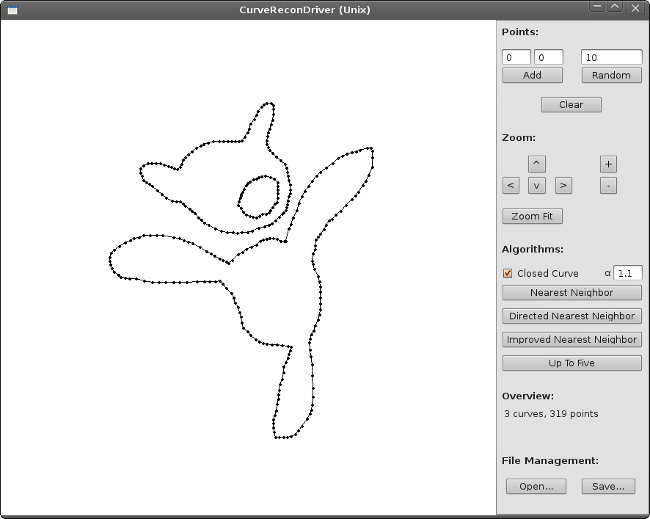
\includegraphics[scale=0.4]{Discussion/newdebugprogram.png}
  \label{fig:gui}\\
  Figure 3.1: GUI of visualization
\end{center}
\end{figure}

\subsection{Nearest Neighbor}
  \label{sub:nn_test_results}
    \textbf{Running time}\\
    We first tested our algorithm on randomly generated points (solely for determining the running time of the algorithm).\\
    The results are given in the Table 3.1 and Figure 3.2.

      \begin{center}
        \begin{tabular}{|p{2.5cm}|p{2.5cm}|}
            \hline
            Points & Seconds\\
            \hline
            \hline
            500 & 0.015\\
            \hline
            1000 & 0.016\\
            \hline
            1500 & 0.047\\
            \hline
            2000 & 0.078\\
            \hline
            5000 & 0.442\\
            \hline
            10000 & 1.669\\
            \hline
            15000 & 4.087\\
            \hline
            20000 & 6.755\\
            \hline
            30000 & 16.552\\
            \hline
            40000 & 27.878\\
            \hline
            50000 & 47,768\\
            \hline
            60000 & 66.16\\
            \hline
            80000 & 108.358\\
            \hline
            100000 & 202.239\\
            \hline
        \end{tabular}
        \label{tab:nn_runningtime}\\
        Table 3.1: A table of our results on testing \textit{NearestNeighbor}
    \end{center}

    \begin{center}
      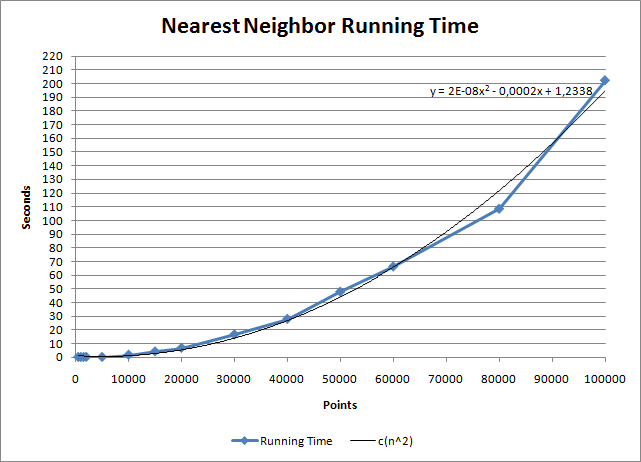
\includegraphics[scale = 0.5]{1NearestNeighbor/nnRuntimegraph.png}\\
      Figure 3.2: Graph of \textit{NearestNeighbor}'s Running Time
      \label{fig:nn_runningtime}
    \end{center}
    This graph tells us that our analysis of the running time (\ref{sub:nearest_neighbor}) is correct: when the number of input points are doubled, the running time is quadrupled $(2^2)$, when they are tripled, the running time is multiplied by roughly $3^2$, etc.\\
    Along with the resulting graph of the test, we introduced a trend line (which is a $n^2$ function fitted to our test results) to show the running time is indeed $O(n^2)$.\\
    So, we can conclude that in practice this algorithm is $O(n^2)$ too.\\ \\ \\
    \textbf{Correct output}\\
    We analyzed a few test-cases that failed giving the correct output.\\
    We give suggestions as to what caused this behavior, and supply possible solutions below.\\

    \noindent An example of a test-case in which \textit{NearestNeighbor} fails is the Heart with 200 points. As you can see in Figure 3.3 there are two places the curve starts zigzagging between points.
    This problem occurs because the correct point in this case is not the nearest neighbor of the previous one. This could be corrected by taking the curve's current direction into account. This way, we could prevent the curve from jumping around.\\
    \noindent Another failed test-case is the Spiral with 91 points (Figure 3.4). Here, we experience the same problem as in the first case, that is, going in the wrong direction because the nearest point is not the correct successor. We also see another problem caused by this: when the spiral is nearly complete, the algorithm picks the points, which haven't been processed yet. In this case those points reside at the other side of the spiral.\\
    \noindent The third test-case is the ``8'' with 364 points (Figure 3.5). The problem here is that is does not intersect. Nearest Neighbor does not make sure there is at least one intersection. So, another thing we should take into consideration is that we need to check for intersections. \\
    \noindent The fourth and last test-case we discuss is the Flat with 178 points. This problem could also be solved by keeping track of the curve's current direction, so that it will not end up zigzagging again (marked in Figure 3.6).\\\\
        \begin{center}
        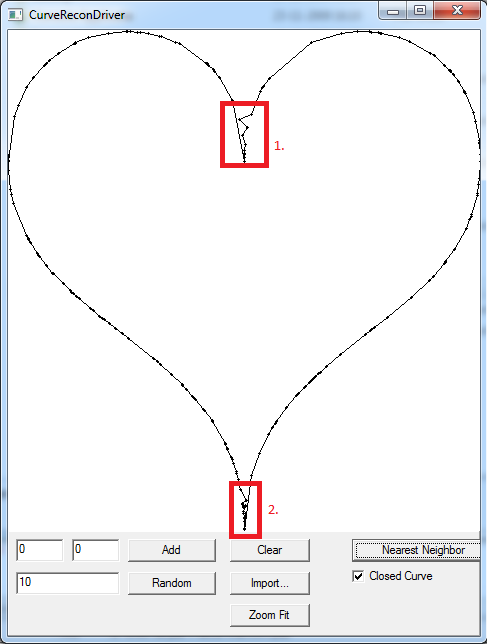
\includegraphics[scale = 0.45]{1NearestNeighbor/nnHeartgraph.png}\\
        \label{fig:nn_incorrectheart}
        Figure 3.3: Incorrect heart
        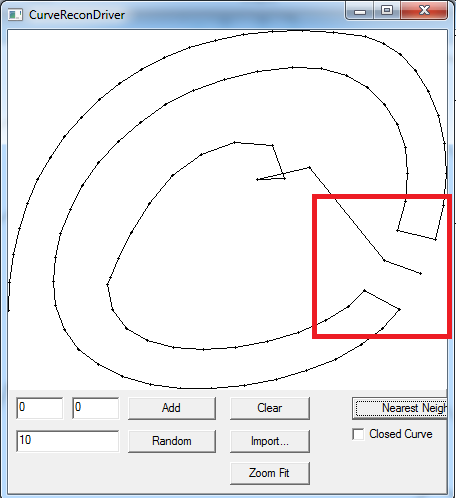
\includegraphics[scale = 0.5]{1NearestNeighbor/nnSpiralgraph.png}\\
        \label{fig:nn_incorrectspiral}
        Figure 3.4: Incorrect spiral
        {\ }\\[1.0cm]
        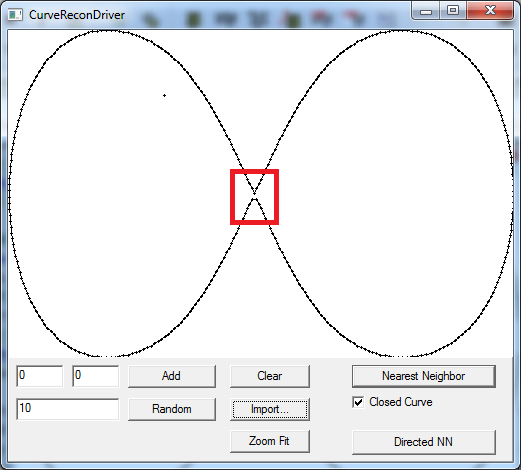
\includegraphics[scale = 0.5]{1NearestNeighbor/nnEightgraph.png}\\
        \label{fig:nn_incorrecteight}
        Figure 3.5: Incorrect eight
        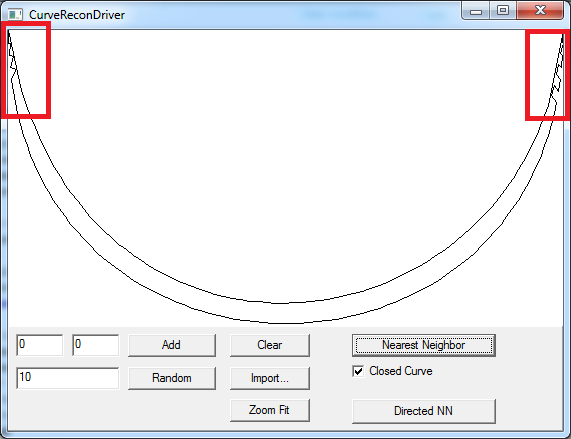
\includegraphics[scale = 0.5]{1NearestNeighbor/nnFlatgraph.png}\\
        \label{fig:nn_incorrectflat}
        Figure 3.6: Incorrect flat
        \end{center}
    \textbf{Conclusion}\\
    From all these test results we can conclude there are a number of things that need improving. We could, for example (as mentioned before), look at the curve's direction, which would fix the zigzagging. We should also check for intersections when the input requires it.

    \subsection{Directed Nearest Neighbor}
  \label{sub:dnn_test_results}
    \textbf{Running time}\\
        To determine the running time of the Directed Nearest Neighbor algorithm, we first tested our algorithm on randomly generated points.\\
        We ran the experiments on a HP Compaq 8510w Laptop with the following specifications:\\
        2,4 GHz Intel Core 2 Duo processor T7700\\
        2 GB memory.
        The results are given in Table 3.2 and Figure 3.7. The constant used by the algorithm was set at $1.5$, meaning the range for \textit{FindPointsInRange} is the length of the last-drawn line multiplied by $1.5$.

        \begin{center}
          \begin{tabular}{|p{2.5cm}|p{2.5cm}|}
              \hline
              Points & Seconds\\
              \hline
              \hline
              500 & 0.015\\
              \hline
              1000 & 0.047\\
              \hline
              1500 & 0.078\\
              \hline
              2000 & 0.14\\
              \hline
              5000 & 0.624\\
              \hline
              10000 & 2.246\\
              \hline
              15000 & 5.414\\
              \hline
              20000 & 9.407\\
              \hline
              30000 & 20.936\\
              \hline
              40000 & 45.864\\
              \hline
              50000 & 63.367\\
              \hline
              60000 & 93.335\\
              \hline
              80000 & 183.772\\
              \hline
          \end{tabular}
          \label{tab:dnn_runningtime}\\
          Table 3.2: Results of testing \textit{DirectedNearestNeighbor}
        \end{center}

        \begin{center}
        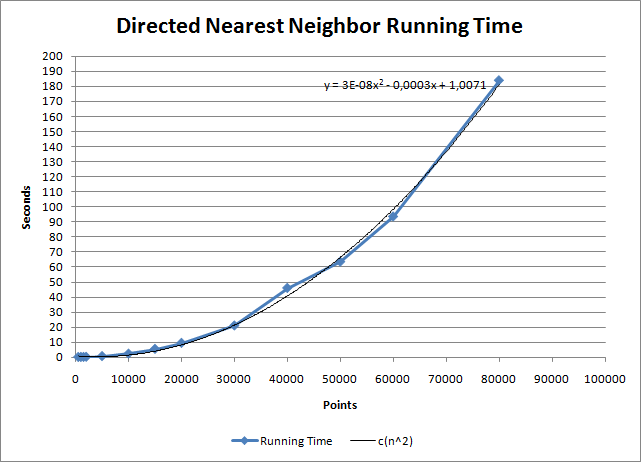
\includegraphics[scale = 0.5]{2DirectedNearestNeighbor/dnnRuntimeGraph.png}\\
        Figure 3.7: Graph of \textit{DirectedNearestNeighbor}'s Running Time
        \label{fig:dnn_runnningtime}
        \end{center}

        \noindent When comparing the above running times to the ones from Nearest Neighbor, we observe this algorithm is indeed a little slower as we have shown in the running time analysis (~\ref{sub:directed_nearest_neighbor}). However, when we introduce a trend line that derives a $n^2$ function from the results, we see that the algorithm is still $O(n^2)$.\\\\
        \textbf{Correct Output}\\
        After testing some of the test-cases, we noticed some of the previous algorithm's problems were now solved. The Flat test-case with 178 points was constructed correctly with the DirectedNearestNeighbor.

        \begin{center}
        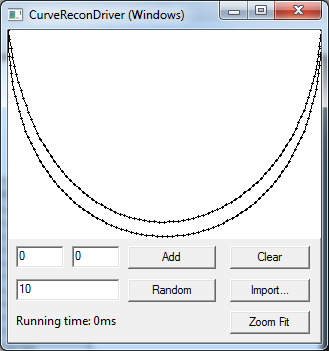
\includegraphics[scale = 0.6]{2DirectedNearestNeighbor/dnnFlatgraph.png}\\
        \label{fig:ddn correctflat}
        Figure 3.8: Correct Flat
        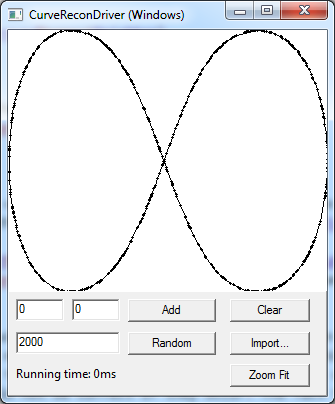
\includegraphics[scale = 0.6]{2DirectedNearestNeighbor/dnnEightGraph.png}\\
        \label{fig:ddn correctflat}
        Figure 3.9: Correct ``8''
        \end{center}
        But we also noticed test-cases still going wrong, this is due to that the algorithm still does not check for intersections when they are needed or not, another possibility is a non-optimal choice of the constant for determine the range. A clear example of this is the Spiral test-case. When we ran this with the above stated constant, we saw that because there were two points really close to each other (see red square in Figure 3.10), it does not choose the point after it correctly. This is because the next line to be drawn is much longer than $1.5$ times the small line between the previous two points.\\
        \noindent Another thing we noticed was that the problem of lines going right through the graph still existed (and maybe even got worse, see Figure 3.11). This is because, now that the algorithm is pickier, more points are left at the end. Since the algorithm wants to connect all points, it picks the ones left at the end.
        A solution for this could be checking for unused points at the end, and then try to insert these point in the correct place.
        \begin{center}
        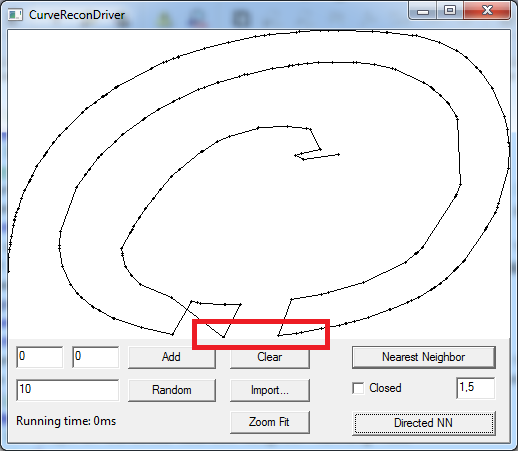
\includegraphics[scale = 0.5]{2DirectedNearestNeighbor/dnnSpiralgraph.png}\\
        \label{fig:dnn_incorrectspiral}
        Figure 3.10: Incorrect Spiral
        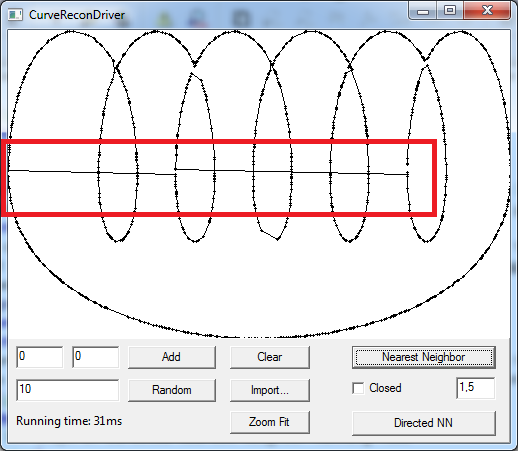
\includegraphics[scale = 0.5]{2DirectedNearestNeighbor/dnnSpringgraph.png}\\
        \label{fig:dnn_incorrectspring}
        Figure 3.11 Incorrect Spring
       \end{center}
        \textbf{Conclusion}\\
        When we look at several incorrect test-cases, we see that we need a better way of picking the range for Find-Points-In-Range. Also, we need to check for unused or incorrectly inserted points at the end. This is needed to make sure the points are inserted correctly and not just connected to each other at the end, messing up the curve. Another thing we could improve on is to look more carefully at the curve's direction, instead of just looking at angles to points in a certain range. Another improvement we should consider is to check for intersections at the end of reconstruction.
\newpage
  \subsection{Improved Nearest Neighbor}
  \label{sub:inn_test_results}
    \textbf{Running time}\\
        The results for our \textit{ImprovedNearestNeighbor} are given in Table 3.3 and Figure 3.12.

        \begin{center}
          \begin{tabular}{|p{2.5cm}|p{2.5cm}|}
              \hline
              Points & Seconds\\
              \hline
              \hline
              500 & 0.016\\
              \hline
              1000 & 0.032\\
              \hline
              1500 & 0.078\\
              \hline
              2000 & 0.156\\
              \hline
              5000 & 1.591\\
              \hline
              10000 & 6.755\\
              \hline
              15000 & 10.935\\
              \hline
              20000 & 17.659\\
              \hline
              30000 & 36.738\\
              \hline
              40000 & 59.202\\
              \hline
              50000 & 107.360\\
              \hline
              60000 & 154.582\\
              \hline
              80000 & 240.034\\
              \hline
          \end{tabular}
          \label{tab:inn_runningtime}\\
          Table 3.3: Results of testing \textit{ImprovedNearestNeighbor}
        \end{center}

          \begin{center}
            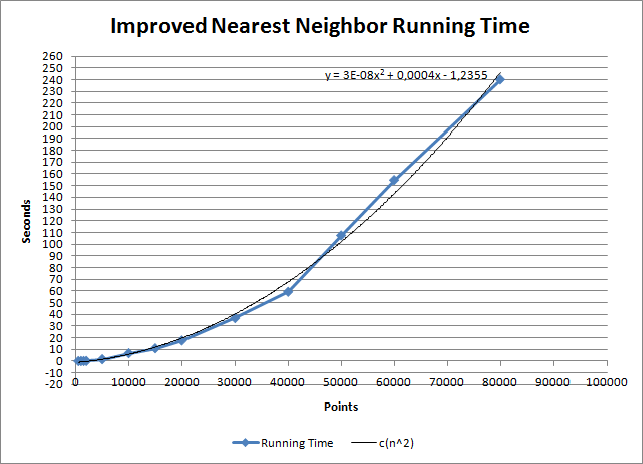
\includegraphics[scale = 0.5]{3ImprovedNearestNeighbor/innRuntimeGraph.png}\\
            Figure 3.12: Graph of \textit{ImprovedNearestNeighbor}'s Running Time
            \label{fig:inn_runnningtime}
          \end{center}

      \noindent The results of the running time are what we expected, again it looks like the algorithm is $O(n^2)$, especially when we introduce the $n^2$ trend line. It may not be that obvious as it was the case with \textit{NearestNeighbor} and \textit{DirectedNearestNeighbor} but we still can conclude using the graph that \textit{ImprovedNearestNeighbor} is $O(n^2)$.
      If we compare the algorithm to \textit{NearestNeighbor} and \textit{DirectedNearestNeighbor}, we see that is slower than \textit{NearestNeighbor}, which is obvious of course since it uses \textit{NearestNeighbor} with an extra function, and faster than \textit{DirectedNearestNeighbor}.\\\\
    \textbf{Correct output}\\
    There were a couple of things that went better with \textit{ImprovedNearestNeighbor} than with \textit{NearestNeighbor}. For example the heart of 128 points (See figure 3.14), which went completely right. Another thing that works much better in Improved Nearest is the following closed curve, when we draw a normal circle with one point at the outside \textit{NearestNeighbor} would fail but the new \textit{ImprovedNearestNeighbor} does not. This is because of the new functionality to insert points at the end, which checks for multiple things which would not be correct if they occur. The fact that the reconstruction of this type of curve has improved is good, since a similar type of curve can be found in several other test-cases we ran.
    See Figure 3.13 to see an example.\\

          \begin{center}
            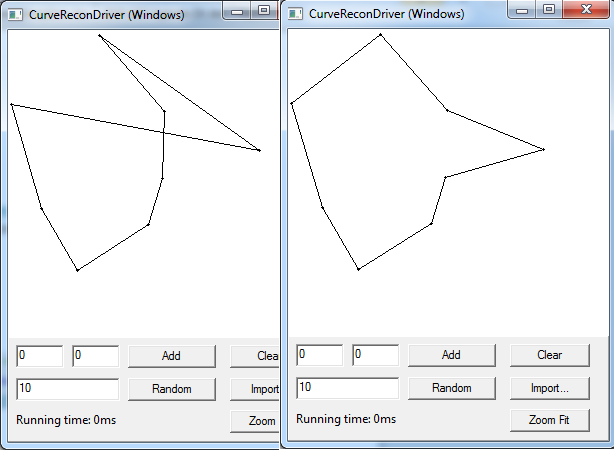
\includegraphics[scale = 0.5]{3ImprovedNearestNeighbor/innPointCirkel.png}\\
            Figure 3.13: Left: Nearest Neighbor Algorithm. Right: Improved Nearest Neighbor Algorithm
            \label{fig:inn_pointcircle}
          \end{center}
\newpage
   \noindent For example one of the test cases which contains this problem; the Heart with 128 points:\\
          \begin{center}
            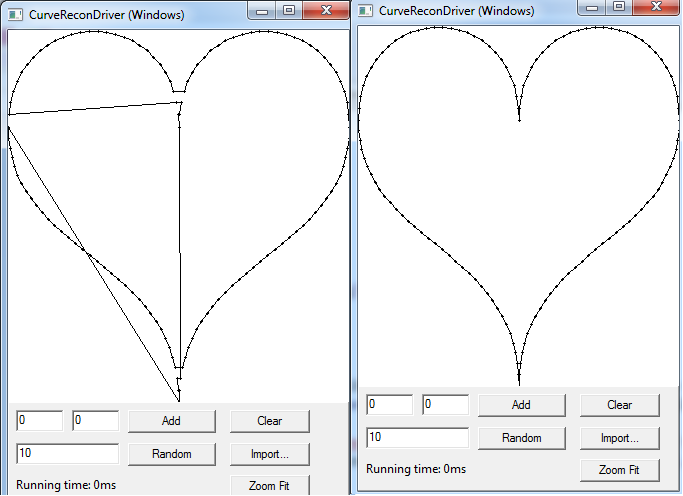
\includegraphics[scale = 0.4]{3ImprovedNearestNeighbor/innHeart.png}\\
            Figure 3.14: Left: Nearest Neighbor Algorithm. Right: Improved Nearest Neighbor Algorithm
            \label{fig:inn_pointcircle}
          \end{center}

    \noindent A test case that still went wrong is the spiral: \\
          \begin{center}
            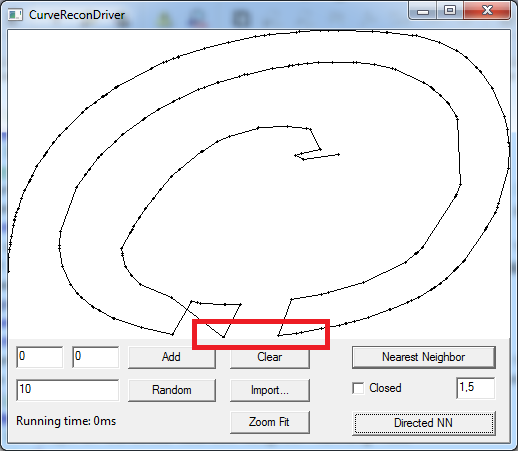
\includegraphics[scale = 0.6]{3ImprovedNearestNeighbor/innSpiral.png}\\
            Figure 3.15: Incorrect Spiral
            \label{fig:inn_pointcircle}
          \end{center}

  \noindent This test case results in the same incorrect reconstruction as with the Nearest Neighbor algorithm. So in this test case the function that inserts lost points at the end didn't have any effect. A suggestion to improve this result would be to add the technic of the Direct Nearest Neighbor to this algorithm. This could result in a much better result.

  \noindent Another test case that went wrong is the Flat with 88 points:\\

            \begin{center}
            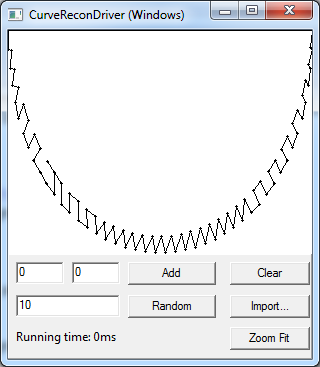
\includegraphics[scale = 0.7]{3ImprovedNearestNeighbor/innFlat.png}\\
            Figure 3.16: Incorrect Flat
            \label{fig:inn_pointcircle}
          \end{center}

  \noindent In this test case we notice some zigzagging, although this is a pretty hard test case since there are only 88 points, the same solution as mentioned above could provide a better reconstruction. Because this test case could probably benefit a lot by checking in which direction the curve is going.\\\\
   \textbf{Conclusion}\\
   We can conclude from the above experiments that Improved Nearest Neighbor really improves a number of problems we first had with the standard Nearest Neighbor algorithm. Especially the function that inserts lost points at the end really provides better results. But still there are a number of test cases that went wrong, to make this number of failing test cases smaller, a combination of the Improved and Directed Nearest Neighbor could maybe be a solution. This could, for example, result in a better reconstruction of the Spiral test case. Another thing that could probably make the reconstructions better is a check for intersections. Since a number of test cases contained a number of intersections which shouldn't be there. For example see the Spiral test case.
   These two suggestions would probably make the Improved Nearest Neighbor even better.
\newpage
    \subsection{Up To Five Sort}
  \label{sub:utfs_test_results}
    \textbf{Running time}\\
    After using the same method as before we got the following results:
        \begin{center}
          \begin{tabular}{|p{2.5cm}|p{2.5cm}|}
              \hline
              Points & Seconds\\
              \hline
              \hline
              500 & 0.015\\
              \hline
              1000 & 5.032\\
              \hline
              1500 & 7.644\\
              \hline
              2000 & 9.812\\
              \hline
              5000 & 24.805\\
              \hline
              10000 & 56.691\\
              \hline
              15000 & 77.330\\
              \hline
              20000 & 105.347\\
              \hline
              30000 & 163.100\\
              \hline
              40000 & 217.278\\
              \hline
              50000 & 281.118\\
              \hline
          \end{tabular}
          \label{tab:utfs_runningtime}\\
          Table 3.4: Results of testing \textit{UpToFiveSort}
        \end{center}

          \begin{center}
            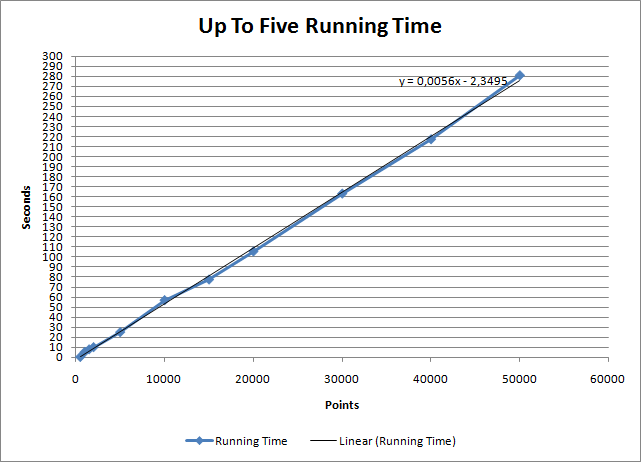
\includegraphics[scale = 0.5]{4UpToFiveSort/utfsRuntimeGraph.png}\\
            Figure 3.17: Graph of \textit{UpToFiveSort}'s Running Time
            \label{fig:utfs runningtime}
          \end{center}

      \noindent If we look at the graph of the running time we see that the algorithm look linear. But if we take in account that the running time determined in section~\ref{sub:up_to_five_sort} is $O(n^3)$ it would be unlikely that the algorithm is $O(n)$. Although the proof of the running time is determined for the worst case this is still awkward. It could of course be that the running time algorithm is really slow getting the form of a $O(n^3)$ function and the tested number of points are a very small part of this. This small part would then look like a linear function. This means that we can conclude that for most cases, in which we use this algorithm, \textit{Up To Five Sort} will have the linear running time $O(n)$.\\\\\\
    \textbf{Correct output}\\
    Since the algorithm uses much of the \textit{Nearest Neighbor} algorithm most incorrect results have similar problems as the \textit{Nearest Neighbor} algorithm.
    Most test cases with an even distance, for example the face with 134 points, or with many points, for example the house with 1000 points, went perfect.

    \begin{center}
        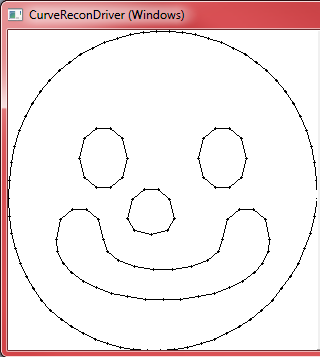
\includegraphics[scale = 0.5]{4UpToFiveSort/utfsFace.png}\\
        \label{fig:utfs_correctface}
        Figure 3.18: Correct Face
        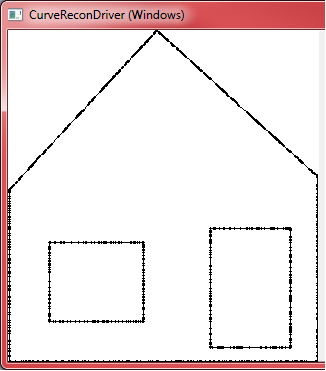
\includegraphics[scale = 0.5]{4UpToFiveSort/utfsHouse1000.png}
        \label{fig:utfs_correcthouse}\\
        Figure 3.19: Correct House of 1000 Points
    \end{center}

    But the algorithm seems to often give a incorrect solution with test cases that don't have much points.
    As an example we took the house with 200 points and 500 points.\\
    \begin{center}
        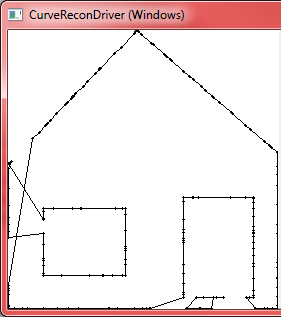
\includegraphics[scale = 0.6]{4UpToFiveSort/utfsHouse200.png}\\
        \label{fig:utfs_incorrecthouse200}
        Figure 3.20: Incorrect House of 200 Points
        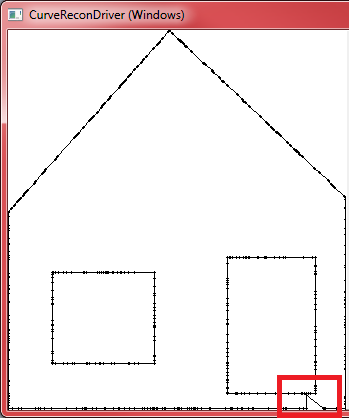
\includegraphics[scale = 0.5]{4UpToFiveSort/utfsHouse500.png}
        \label{fig:utfs_incorrecthouse500}\\
        Figure 3.21: Incorrect House of 500 Points
    \end{center}
    The first test case does not do quite well, the one of 500 points does much better except at the marked (red square in figure) section. A solution to both these problems could be checking for the direction in which the curve should go. The correctness of the reconstruction of the house with 200 points should increase although it is still difficult to determine the range in which you look for the direction the curve should go too, since there are several curves. The house with 500 points would probably be totally correct.\\
    Another test case we will be looking at is the plus test case with 120 points.

          \begin{center}
            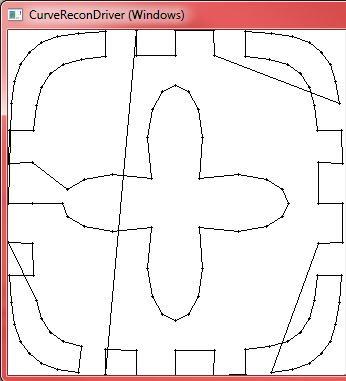
\includegraphics[scale = 0.7]{4UpToFiveSort/utfsPlus128.png}\\
            Figure 3.22: Incorrect Plus
            \label{fig:utfs incorrect plus}
          \end{center}
    We see similar problems as with the above mentioned test cases but also intersections which of course should not occur. A solution to this new problem would be some way to remove the intersections afterwards just like in the \textit{Improved Nearest Neighbor} algorithm.\\ \\ \\
   \textbf{Conclusion}\\
   From the above results we can conclude that the algorithm does give good results for most test cases although there are a couple of things that could be improved. For example taking some techniques we used in \textit{Directed Nearest Neighbor} and \textit{Improved Nearest Neighbor}, like checking the direction in which the curve is going. But these techniques are probably more difficult to insert because there are multiple curves. Since it would be much more difficult to determine the range in which you search for the next point.

\section{Concluding remarks}
\label{sec:Remarks}
We have learned how to implement and test an algorithm. From these test we have enhanced our original algorithm. We have also learned that the solution to any problem is in essence a ``hit or miss''. An engineer must have the right idea at the right time with the right skills to solve a problem. Our first approaches, using a $k$D-tree and making a backtracking algorithm were the wrong ideas. The first because it was too complex to implement, the second because the practical running time was worthless (caused by both the large stack problems of FreePascal and the properties of any backtracking algorithm ).\\
In the end, we have decided to use more simple algorithms to achieve the expected results. We began with implementing a Nearest Neighbor algorithm, which has a running time of $O(n^{2})$, so it was pretty fast. When we tested this algorithm it turned out this was not enough to solve the problem of curve reconstruction. There was a lot of zigzagging in the resulting figures and lines from one end of the figure to the other. The last problem was caused by the fact that when \textit{NearestNeighbor} is about to connect the last point it checks whether all points in the input array are used, if this is not the case it connects them, which can result in such lines.\\


Therefore, the next idea was to improve this algorithm by looking at the direction of the curve constructed so far. We developed functions to find points within a certain range from the current point, and a function to determine which of the just found points differs the least from the current direction. To get rid of the lines running from one end of the figure to the other caused by skipping points, we insert these skipped points into the solution array at the right spot in the end. This way no lines from one end of the figure to the other are possible. We called this algorithm \textit{DirectedNearestNeighbor}, because its main functionality is looking at direction. This algorithm also has an running time of $O(n^{2})$, so it was still fast enough to solve the problem within the amount of time that was given, namely 5 minutes. From the test results of this algorithm we concluded that in most cases the zigzagging was gone, but the most resulting figures were still not what we wished for, but when we ran \textit{DirectedNearestNeighbor} on self-intersecting curves it gave good results. So we decided to use this algorithm for self-intersecting curves.\\
For the other three types of curves we have improved \textit{NearestNeighbor}. This new algorithm, called \textit{ImprovedNearestNeighbor} still inserts skipped points, but also has a new function to make open curves. This is done by deleting the longest edge after constructing a closed curve. Also this algorithm still has a running time of $O(n^2)$. The results were satisfying for the open and closed curve test-cases, so we decided to use this algorithm for those two types.\\
That left us with one type of curve: the up-to-5 curve. For this case we designed a new algorithm still based on \textit{NearestNeighbor} without checking whether all points occur in the solution array. When \textit{NearestNeighbor} has constructed a curve, this curve is stored in a solution array and the remaining points in the set are used to construct another curve, this continues until all points are used. When at the end more than $5$ curves were created the smaller curves are inserted into the closest big curve, until less than $5$ curves occur in the solution. This way we can guarantee no more than $5$ curves are returned. Though the worst-case running time of this algorithm, called \textit{UpToFiveSort}, is $O(n^{3})$ it turns out on the average case its linear! The results were very good, so we did not need to improve this algorithm anymore.\\
Of course there is always room for improvements on all the algorithms we made. One of them is to check for intersections; in a self-intersecting curve a check is needed wether it contains at least one intersection, on the other hand in an open, closed or up-to-five curve no intersections are allowed. If this check is added you can guarantee that the solution given by the algorithms always satisfies the conditions of the different types of curves.\\

\bibliographystyle{plain}
\begin{thebibliography}{9}
  \bibitem{algorithms}  
    T.H. Cormen, C.E. Leiserson, R.L. Rivest and C. Stein. 
    \textit{Introduction to Algorithms} (2$^{nd}$ edition). 
    MIT Press, 2001.
  \bibitem{geometry}
    M. de Berg. 
    \textit{Computational Geometry: Algorithms and Applications} (3$^{rd}$ edition). 
    Springer, 2008.
  \bibitem{kd-trees}
    Andrew Moore. 
    Efficient Memory-based Learning for Robot Control. 
    \textit{An intoductory tutorial on kd-trees}. 
    pages 6-1 - 6-18, 1991.
\end{thebibliography}

\end{document}
